\documentclass[a4paper]{article}

%% Language and font encodings
\usepackage[english]{babel}
\usepackage[utf8x]{inputenc}
\usepackage[T1]{fontenc}
\usepackage{subfig}
\usepackage{multirow}
\usepackage{array}
\usepackage[noend]{algpseudocode}
\usepackage{algorithm}
\usepackage{pdfpages}
\usepackage{amsmath}


%% Sets page size and margins
\usepackage[a4paper,top=3cm,bottom=2cm,left=3cm,right=3cm,marginparwidth=1.75cm]{geometry}

%% Useful packages
\usepackage{amsmath}
\usepackage{graphicx}
\usepackage[colorinlistoftodos]{todonotes}
\usepackage[colorlinks=true, allcolors=blue]{hyperref}

\newcommand\descitem[1]{\item{\bfseries #1}\\}

\title{Sampling Multiple Elements from Bloom Sample Tree and Detecting Communities In Highly Overlapping Graphs using Bloom Filters}
\author{Pratham Shah \and Shubham Jain}

\begin{document}
\maketitle

\section{Introduction}
Bloom Sample Trees \cite{sengupta:2017} can be very effectively used to represent a namespace using Bloom Filters. In this paper, we present solutions of three different problems, with the help of Bloom Sample Trees. 


\section{Sampling Multiple Elements}
To sample multiple elements from a set stored in a Bloom Filter, we can extract an element multiple times from a Bloom Filter as explained in \cite{1}. However, this method can be very slow when the namespace and number of elements to be samples is very large. Thus, we look at different approaches to sample multiple elements from a set represented as a Bloom Filter.
\subsection{Algorithm}
We describe different approaches to extract multiple samples from Bloom Sample Tree apart from extracting one sample from a Bloom Sample Tree multiple times.
\subsubsection{Approach 1 (Thread Pool)}
\begin{enumerate}
  \item A fixed number of threads are created.
  \item To sample n elements, a job queue is created, and the task is added to the job queue.
  \item Whenever a thread is idle in the thread pool, it fetches a job from job queue and samples an element independently.
\end{enumerate}


\subsubsection{}{Approach 2 (Thread spawning)}

In this approach, we start with the root node, compute the estimated number of elements in the intersection of the query set and both the children, if:
\renewcommand{\theenumi}{\alph{enumi}}
\begin{enumerate}
   \item Estimates for both children are zero; then we tell the parent node that no elements were found.
   \item One estimate shows some elements, then we create a thread for the child node and search along that path.
   \item Both the estimates show some elements; we create two threads for the children and sample elements from each path, some elements proportional to the estimated number of elements in the intersection of in both the children respectively.
   \end{enumerate}
On reaching a leaf node, the required number of elements are sampled.


\subsubsection{Approach 3 (Combining Approach 1 and 2)}
\renewcommand{\theenumi}{\arabic{enumi}}
\begin{enumerate}
\item    Here we create some threads, equal to the number of nodes in bloom sample tree and if there are more nodes than a threshold, then we use a fixed number of threads.
\item  Assign each thread to the number of nodes equal to ratio, where ratio=nodes/threads.
\item    Every thread has access to pointers to it's assigned nodes.
\item    Every node has a state array which stores number of elements to be sampled at that node.
\item    Whenever a node has non-zero state array it will divide the samples proportional the estimated number of intersections of query bloom filter with left and right nodes.
\item    Parent thread will update the state array of child nodes according and notify that they have some elements to be sampled.
\item    It keeps happening till we reach leaf node where leaf samples number of elements equal to value in its state array and store it in the result array.
\end{enumerate}


\subsection{Experimental Evaluation}
In this section, we describe the experiments we did with different approaches using a static namespace. We compared running time of different approaches to generating a single sample the required number of times.

\subsubsection{Setup}
We used a static synthetic namespace to compare the running time of the different approaches. We varied our namespace from $10^5$ to $10^7$. We also varied the number of samples to be generated from $1000$ to $10000$.In the combined approach, we have used 256 threads for the below experiments. \newline
\textbf{Query Sets} In the experiments we performed; we generated query sets uniformly at random from the entire namespace.
\newline
\textbf{Algorithms} We compared the running time of approaches $2$ and $3$ and compared it to running time of generating a single sample the required number of times.
\newline
\textbf{Metrics} We report the running time of algorithms by running them multiple times and taking an average of the running times.


\subsection{Results}
Figure 1 shows the average time taken to sample multiple elements from a set using a Bloom Sample Tree using different approaches. The experiment demonstrate that creating multiple threads in advance and then using each to handle multiple nodes is the best strategy of the proposed ones.
\begin{figure}[h!] 
\centering
\begin{tabular}{cccc}
\subfloat[$m=10^4$, $n=10^4$, $M=10^5$]{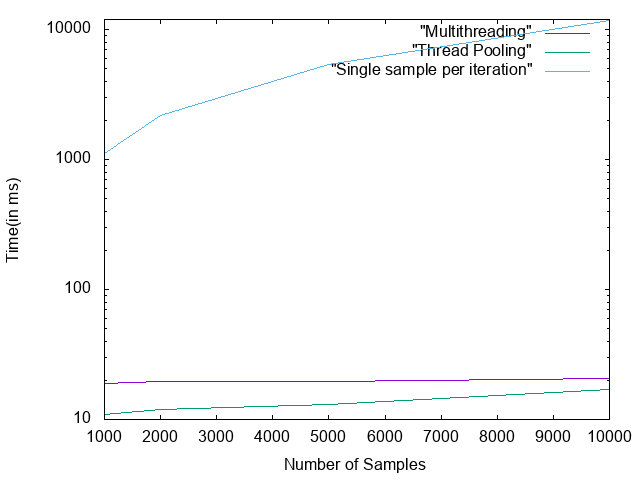
\includegraphics[width=0.5\textwidth]{plot5.png}} 
\subfloat[$m=10^5$, $n=10^4$, $M=10^6$]{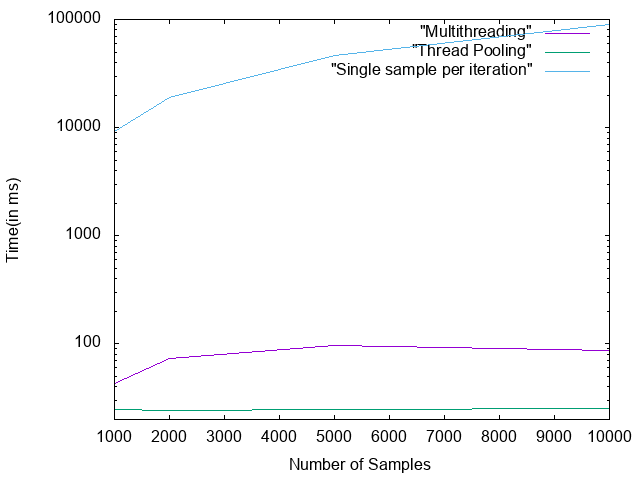
\includegraphics[width=0.5\textwidth]{plot6.png}}\\
\subfloat[$m=10^6$, $n=10^4$, $M=10^7$]
{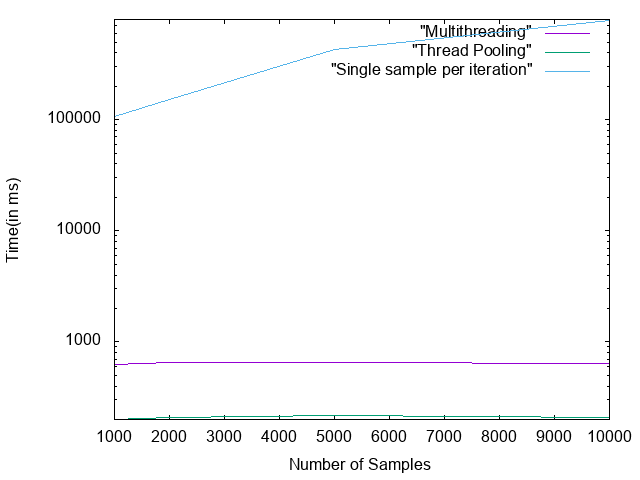
\includegraphics[width=0.5\textwidth]{plot7.png}}
\subfloat[$m=10^6$, $n=10^4$, $M=10^8$]
{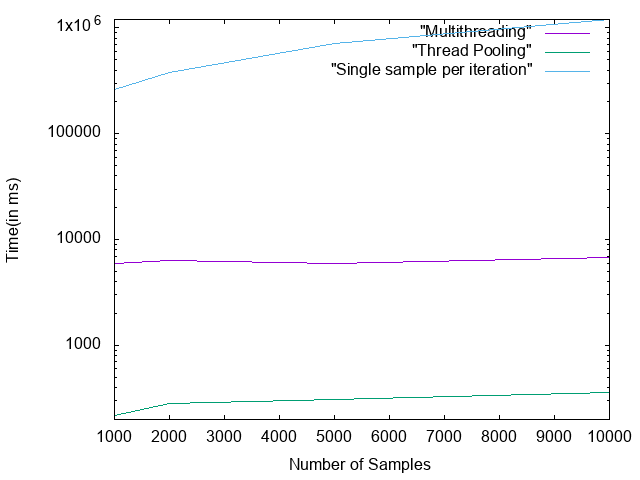
\includegraphics[width=0.5\textwidth]{plot8.png}}
\end{tabular}

\caption{\label{fig:plot}Time taken for different approaches}
\end{figure}


\section{Calculating Set Difference Among Sets Stored in Bloom Filters}

Bloom Filters {\cite{2}} are data structures that can efficiently answer set-membership queries.  Swamidass \& Baldi (2007) {\cite{3}} demonstrated how the size of union and intersection of two sets represented using Bloom Filters can be estimated. However, a very fundamental problem of calculating the set difference between two sets stored as Bloom Filters remains solved. In this paper, we give a method to estimate elements in the set difference between two sets represented as Bloom Filters. \newline
\textit{Problem Statement}. If we are given two sets $S1$ and $S2$ from a namespace $U$ stored in Bloom Filters $B1$ and $B2$ respectively, then we try to estimate elements that are in $S1$ but not in $S2$. \newline
$Solution Overview.$ We exploit Bloom Sample Tree {\cite{1}} to represent the entire namespace. We go down the tree estimating the number of common elements between nodes of the tree and $S1$ and $S2$. If no common element with $S1$ is found, search along that path is pruned, if no common element with $S2$ is found, the node is added into the result and if there are common elements with both sets are found, we move a level down on the path.

\subsection{Algorithm}
The following algorithm is used to estimate elements in the set difference among two sets $S$, and $C$ represented as Bloom Filters using Bloom Sample Tree $B$ which represents namespace where $B_{ij}$ represents $j^{th}$ node of $i^{th}$ level.

\begin{algorithm}
\caption{$Set\_diff (B_{ij}, S, C)$}
\begin{algorithmic}[1]
\Procedure{Set\_diff}{$B_{ij}, S, C$}
 \If{$isLeaf(B_{ij})$}
    \State \textbf{return} all elements of $B_{ij}$ that are in $S$ and not in $C$
  \ElsIf{$B_{ij} \cap S = \phi$}
    \State  \textbf{return} $\phi$
     \ElsIf{$B_{ij} \cap C = \phi$}
    \State  \textbf{return} $S$
    \Else 
    \State
    \textbf{return} $Set\_diff (B_{i+1,2j}, S, C) \cup Set\_diff (B_{i+1,2j+1}, S, C)$
  \EndIf
\EndProcedure
\end{algorithmic}
\end{algorithm}
\begin{algorithm}
\caption{$Set\_difference (B_{ij}, S, C)$}
\begin{algorithmic}[1]
\Procedure{Set\_difference}{$B_{ij}, S, C$}
 \State 
 \textbf{return} $Set\_diff (B_{0,0}, S, C)$
\EndProcedure
\end{algorithmic}
\end{algorithm}


\begin{figure}[h!] 
\centering
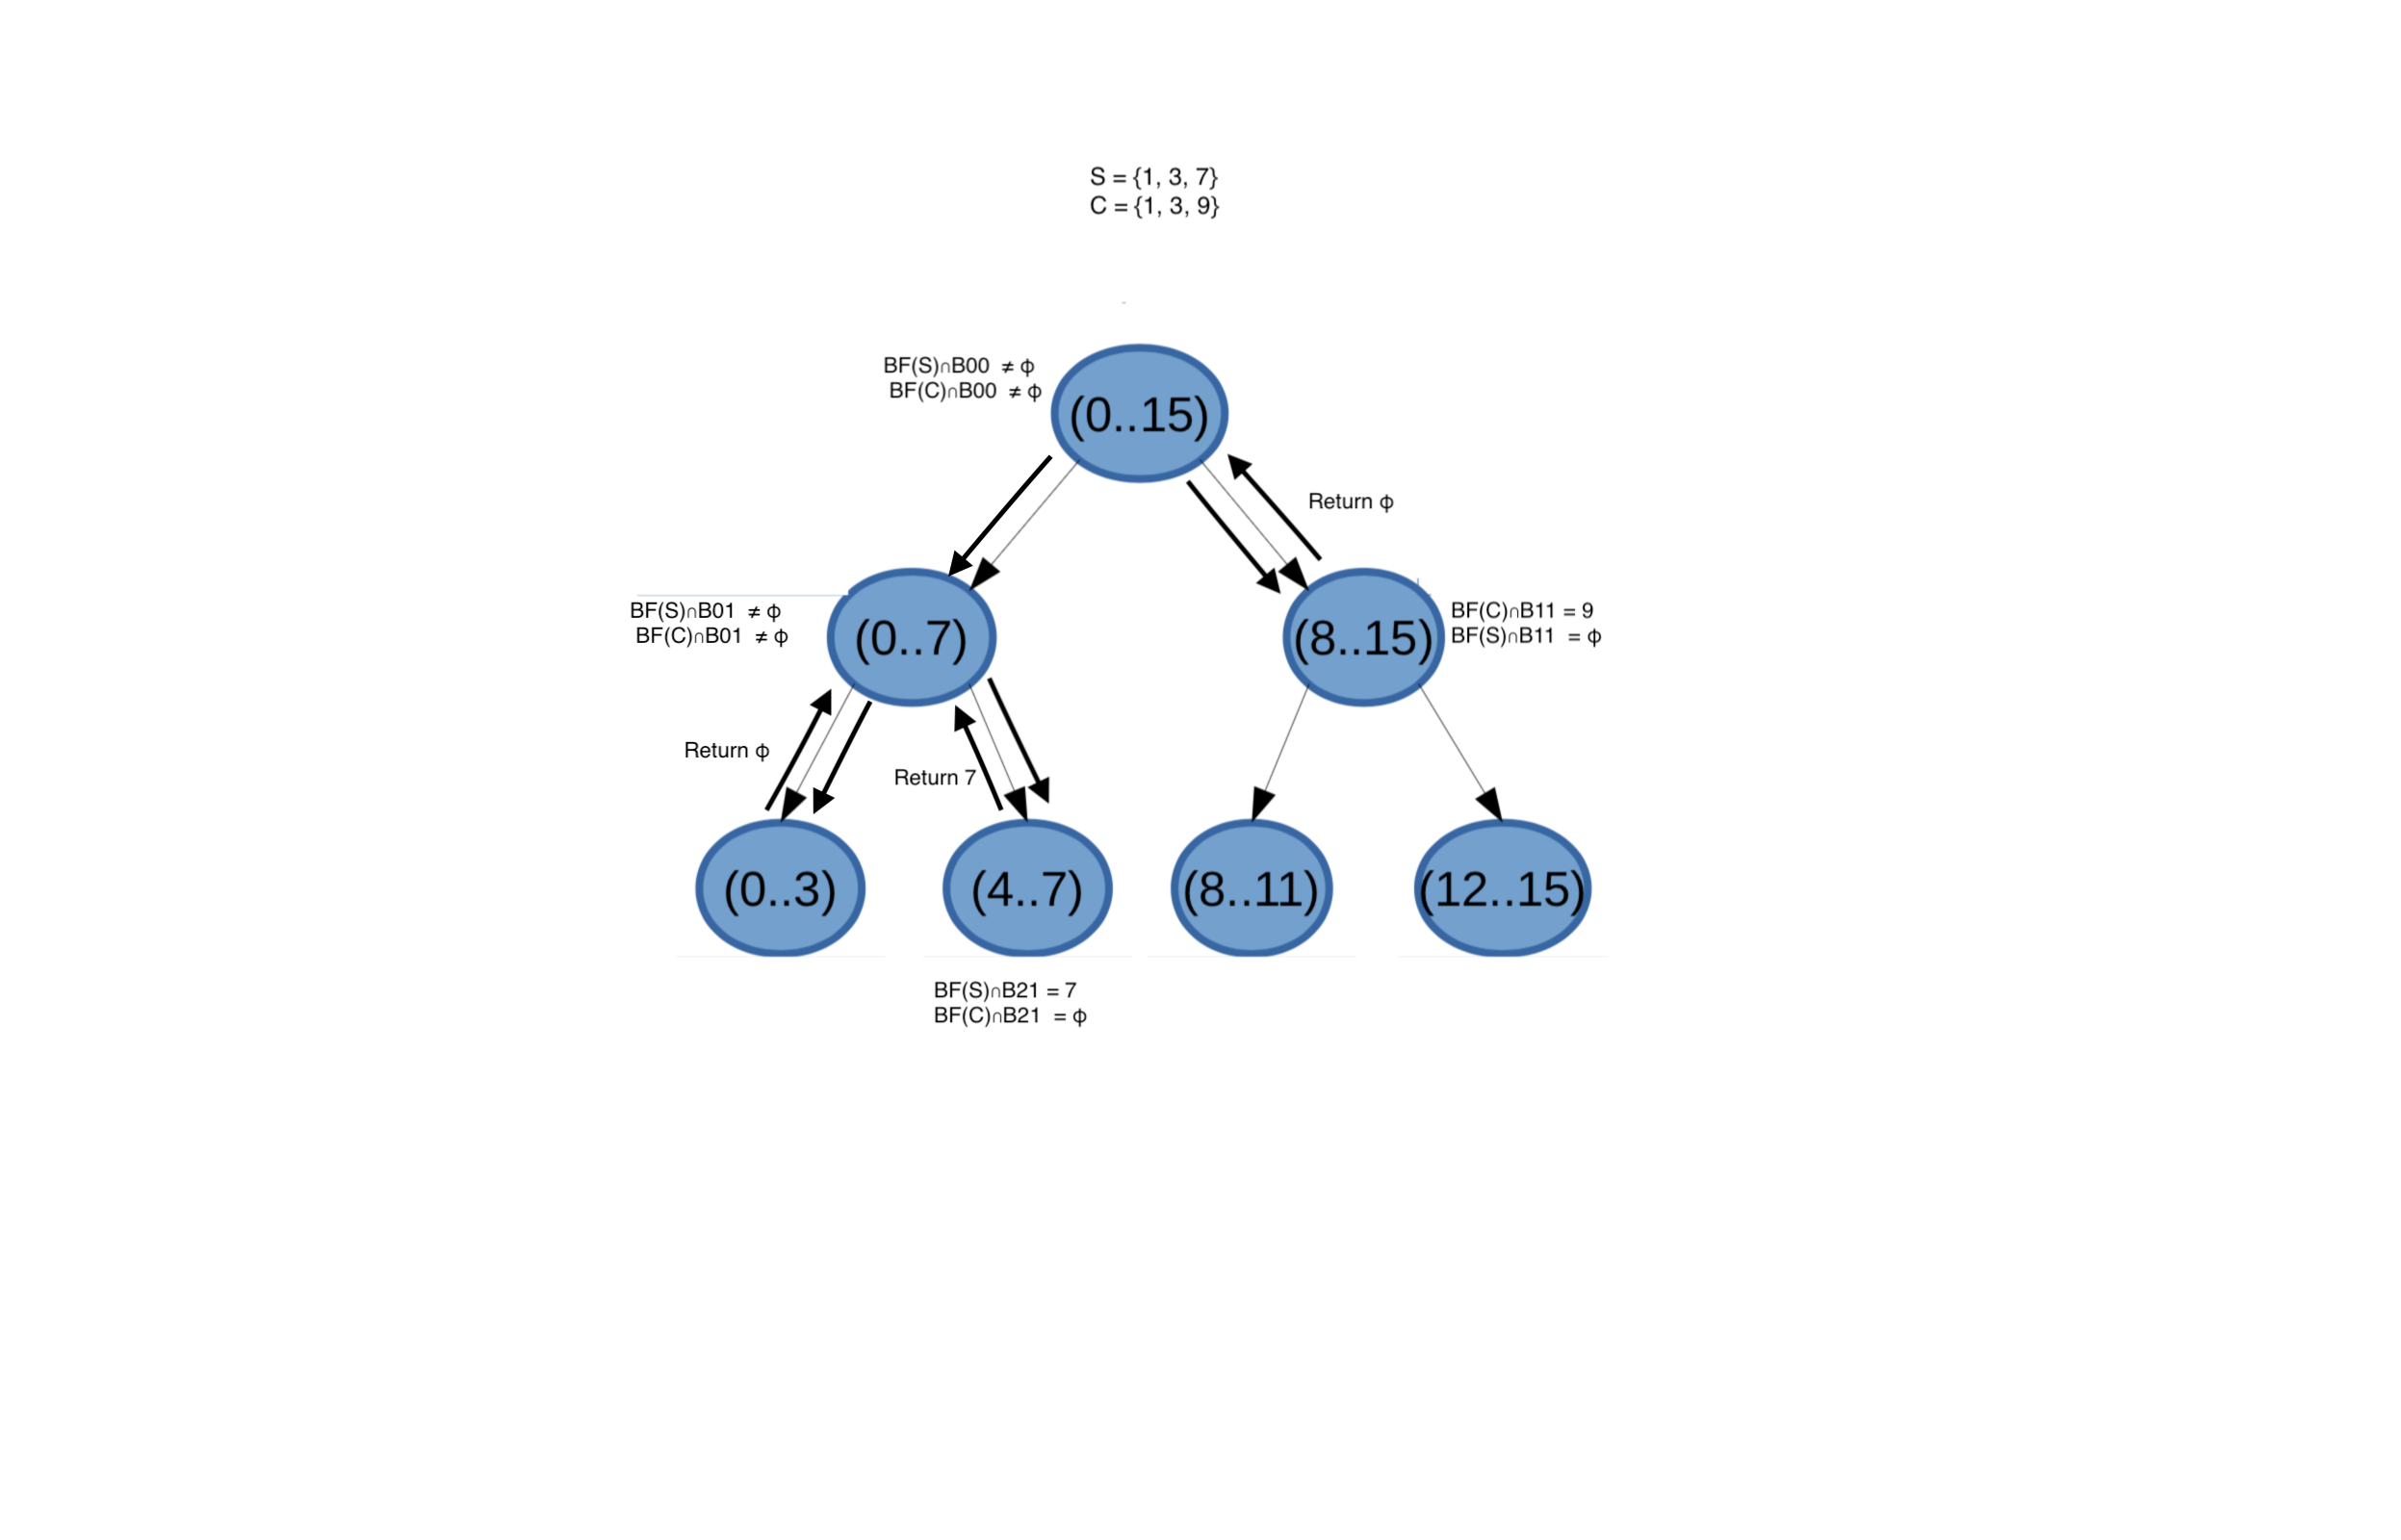
\includegraphics[width=0.6\textwidth]{sd.png}
\caption{\label{fig:Set Difference}Calculation of set difference}
\end{figure}



\subsection{Experimental Setup}
\begin{enumerate}
 \item Namespace (M) = $[1, 2, 3, ... 10^6]$
 \item Bloom filter size (m) = 50000
 \item Both sets A and B are sampled uniformly at random without replacement from M.
 \item In AResults, size of B is fixed to 500, and the size of A is varied in (10,20,40,80,160,320,640,1280).
 \item Similarly in BResults, size of A is fixed to 500, and size of B is varied in the same set.

\end{enumerate}

$A-B$ was calculated independently keeping the sizes of one set constant and varying the other. Precision, recall and F1-score were calculated for the experiments

\subsection{Results}
Figure 3 describes precision, recall and F1-score variation in calculating the Set difference between two sets.

\begin{figure}[h!] 
\centering
\begin{tabular}{cccc}
\subfloat[$A-B$ with varying $B$ and constant $A$]
{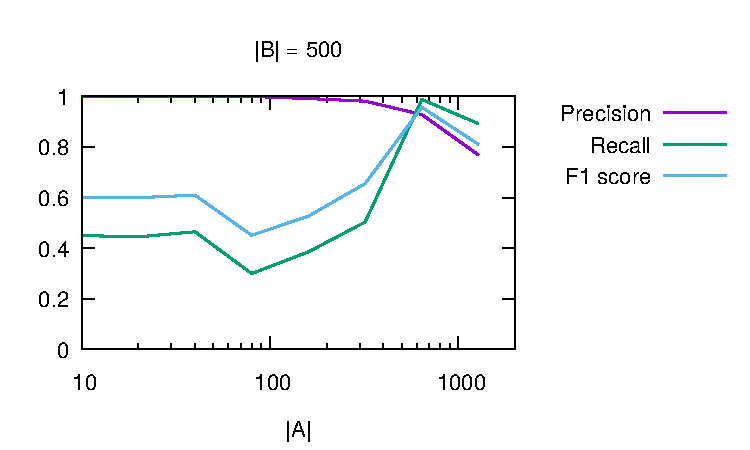
\includegraphics[width=0.5\textwidth]{AResults.pdf}} 
\subfloat[$A-B$ with varying $A$ and constant $B$]
{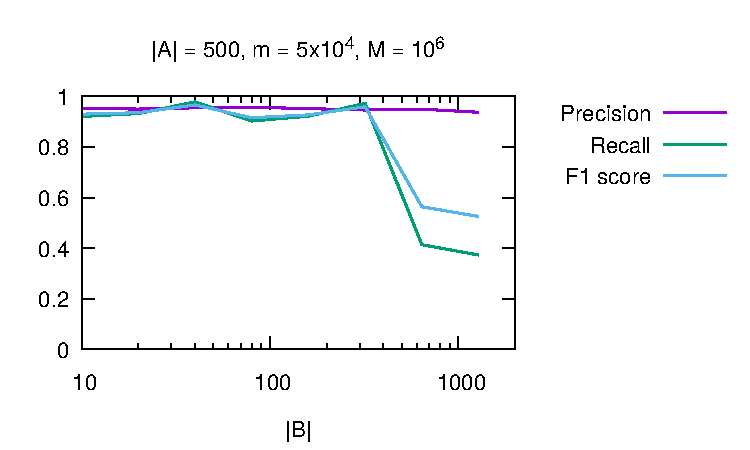
\includegraphics[width=0.5\textwidth]{BResults.pdf}}
\end{tabular}

\caption{\label{fig:plot}F1-score for Set difference}
\end{figure}












\section{Detection of Communities in Overlapping Graphs}
Communities are a significant part of a lot of networks like social networks as they tell about relationships between different people in the network. In the real world, it can be seen that a single entity may belong to multiple communities. Thus, it can be an important problem to find communities in overlapping graphs. \newline

One might find it useful to save a network as a collection of adjacency lists stored as Bloom Filters as it can be very space efficient. Here, we propose a method to detect communities in overlapping bloom graphs (graphs represented as adjacency lists, stored as Bloom Filters).\newline

\textit{Problem Statement}. Given a Graph $G$ with vertices $V_1, V_2,...,V_n$  and edges $E_1, E_2,...,E_m$, find all the communities $C_1, C_2,...,C_l$ in the graph. \newline
\textit{Solution Overview}. Given an undirected network G = (V, E) where V represents the set of vertices in the graph and E the set of edges. Let us denote shell nodes as set S and community node as set C.Any vertex v $\epsilon$ S has at least one neighbour in C and v $\not\in$ C. \newline
To detect communities, we are going to expand around a seed node. The algorithm uses a fitness measure. Fitness Measure value describes how well-connected community is. The algorithm only adds those nodes to the community which increases community fitness.\newline
\textit{Alpha-Measure}\cite{lancichinetti:2008}. It is a community fitness measure we used in our algorithm for measuring community fitness.\newline
$K_{in}$ denotes the sum of in-degree and out-degree of the nodes in the community.
$K_{out}$ denotes the sum of out-degree of the nodes whose one end of the edge is in the community, and another end is connected with a node outside community.\newline
$\alpha$ is a hyper-parameter which can be adjusted accordingly.

\begin{align*}
F_S 
&= \frac{k_{in}^S}{(k_{in}^S+k_{out}^S)^\alpha}  
\end{align*}





\subsection{Algorithm}
The following algorithm is used to generate communities from an overlapping Bloom Graph.

\begin{algorithm}
\caption{$Community\_detection (seed)$}

\begin{algorithmic}[1]
\Procedure{Community\_detection}{seed}
\State $ size\gets 1$
\State $ b\gets seed$        \Comment{Community Bloom Filter}
\State $ numCandidates\gets 100$        \Comment{Hyper-Parameter can be changed as per need}
\State $ measure_b\gets 0$ \Comment{conductance or alpha-measure}
\While{True}
\State $candidate\_list\gets\phi$\Comment{This is a list of tuples}
\For{(j = 1 to min(numCandidates, size)}
\State sample element u from Bloom filter b
\State sample element v from adj(u)
\If {v in b} 
\State continue
\EndIf
\State $t \gets$ numOnes in $adj(v) \cap b$
\State $candidateList\gets candidatelist.append((v,t))$ \Comment{ append tuple (v,t) to the list}
\State sort candidateList by the second element in each tuple
\State truncate candidateList to top K
\State put candidateList in another Bloom filter C
\If{inserting c into b increases measure\_b}
\State $b\gets b \cup c$
\State $size \gets size + K$
\State $update measure\_b$
\Else \State break
\EndIf
\EndFor
\EndWhile
\State \textbf{return} b
\EndProcedure
\end{algorithmic}
\end{algorithm}



\subsection{Experimental Setup}
\begin{enumerate}
 \item Graph is generated using CKB generator \cite{10.1007/978-3-319-05401-8_19}. Parameters used are as mentioned in Figure 4.
 \item Graph is undirected and communities are highly overlapping.
 \item Number of Nodes in Graph = 100,000 and 1,000,000.
 
 \item F-score of a community predicted using the above algorithm are calculated with the communities in ground truth.
 \item We have used alpha = 0.75 (hyper-parameter) and m = 2*number of nodes.
 \item The following algorithms were tested:
 
 \begin{enumerate}
 
  \descitem{Page Rank Nibble \cite{PRN}} 
 
 \descitem{LFM \cite{lancichinetti:2008}} % Let
%us suppose that we have covered a subgraph $G$ including node A. Initially, $G$ is identified with node A. Each iteration of the algorithm consists of the following steps:
% \begin{enumerate}
%\item a loop is performed over all neighboring nodes of $G$ not included in $G$;
%\item the neighbor with the largest fitness is added to $G$, yielding a larger subgraph $G'$;
%\item the fitness of each node of $G'$ is recalculated;
%\item if a node turns out to have negative fitness, it is removed from G, yielding a new subgraph $G′′$;
%\item if 4 occurs, repeat from 3, otherwise repeat from 1 for subgraph $G′′$.
%\end{enumerate}
  \descitem{GCE \cite{lee:2010}} %It calculates cliques from the entire graph and then uses them as seeds and greedily adds nodes from surroundings to the community until fitness function increases.%
  \descitem{1 node expansion} We expand community using a seed node. We sample neighbouring nodes which have an edge to the community. We find the fitness function after adding each of the neighbouring nodes individually to the community and add the node to the community which causes the maximum increase in the fitness function. We stop the algorithm when no more nodes can be added to the community which increases fitness function.
  \descitem{Randomized with lists} We expand community using a seed node. We sample k nodes which have an edge to the community. We find the fitness function after adding each of the k nodes individually to the community and add the node to the community which causes the maximum increase in the fitness function. We stop the algorithm when no more nodes can be added to the community which increases fitness function.     
 
\end{enumerate}
 
\end{enumerate}

\begin{figure}[h!] 
\centering
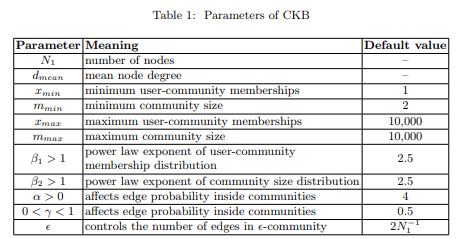
\includegraphics[width=0.6\textwidth]{ckb.PNG}
\caption{\label{fig:Parameters}Parameters used to generate graph}
\end{figure}


\subsection{Results}
\begin{enumerate}
 \item Community is predicted using above algorithm around a seed node.
 \item The predicted community's F-score is calculated with the ground truth communities.
 \item Below results are collected as an average of 10 experiments.
 
 


\begin{center}
\captionof{table}{Experiment 1 (100,000 nodes)}  
 \begin{tabular}{||c c c c c c c||} 
 \hline
 Algorithm & k & Memory(MB) & Precision & Recall & F-Score & Time(ms)\\ [0.4ex] 
 \hline\hline
 
 Page Rank Nibble & - & 60.78 & 0.06 & 0.16 & 0.05  & 35.31\\ 
 \hline
 LFM & - & 60.78 & 0.6 & 0.11 & 0.05 & 1,298.02\\ 
 \hline
 GCE & - & 937.45 & 0 & 0.33 & 0 & \\ 
 \hline
 1 Node Expansion & - & 1.11 &0.58 & 0.54 & 0.53 & 1,416.47\\
 \hline
 Randomized with Lists & 20 & 1.13 & 0.67 & 0.29 & 0.40  & 409.57\\
 \hline
 Randomized with Lists & 30 & 1.12 & 0.81 & 0.42 & 0.5 & 214.49 \\
 \hline
 Randomized with Lists & 40 & 1.14 & 0.64 & 0.44 & 0.51  & 854.58 \\  
 \hline
 Randomized with Bloom Filter & 20 & 0.89 & 0.80 & 0.37 & 0.50 & 221,855.68\\  
 \hline
 Randomized with Bloom Filter & 30 & 0.89 & 0.65 & 0.40 & 0.48  & 265,731.79\\  
 \hline
 Randomized with Bloom Filter & 40 & 0.89 & 0.80 & 0.42 & 0.55  & 203,679.22\\  
 \hline
\end{tabular}
\end{center}





\begin{center}
\captionof{table}{Experiment 2 (1,000,000 nodes)}  
 \begin{tabular}{||c c c c c c c||} 
 \hline
 Algorithm & k & Memory(MB) & Precision & Recall & F-Score & Time(ms)\\ [0.4ex] 
 \hline\hline
 GCE &   &  &  &  &  & \\ 
 \hline
 1 Node Expansion & - & 11.16 &0.51 & 0.47 & 0.48 & 290.30\\
 \hline
 Randomized with Lists & 20 & 11.17 & 0.53 & 0.29 & 0.34 & 407.20\\
 \hline
 Randomized with Lists & 30 & 11.18 & 0.58 & 0.48 & 0.52 & 857.14\\
 \hline
 Randomized with Lists & 40 & 11.18 & 0.76 & 0.49 & 0.58 & 526.77\\  
 \hline
 Randomized with Bloom Filter & 20 & 8.83 & 0.71 & 0.38 & 0.48 & 753,793.62\\  
 \hline
 Randomized with Bloom Filter & 30 & 8.83 & 0.75 & 0.50 & 0.59 & 588,873.63\\  
 \hline
 Randomized with Bloom Filter & 40 & 8.83 & 0.67 & 0.45 & 0.53 & 1,531,642.51\\  
 \hline
\end{tabular}
\end{center}

\item 
The graph below represents how community size varies with $\alpha$ (with number of samples: 40, number of nodes: 100K and size of bloom filter: 200K).

\begin{figure}[h!] 
\centering
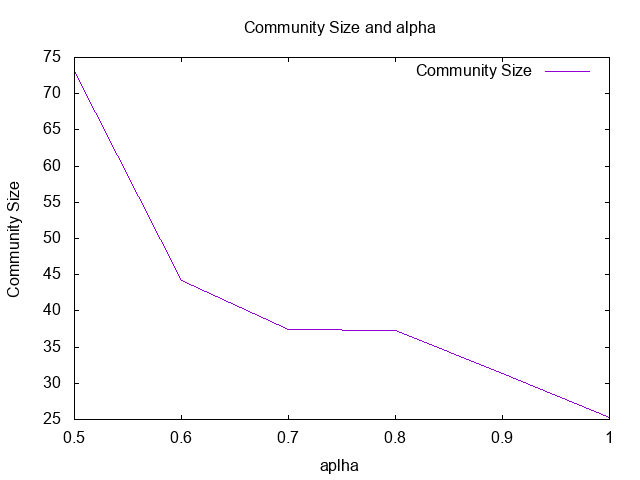
\includegraphics[width=0.6\textwidth]{Community Size.png}
\caption{\label{fig:Community Size and $\alpha$}Community Size and $\alpha$}
\end{figure}


\item 
The graph below represents how F1 score, precision and recall vary with $\alpha$ (with number of samples: 40, number of nodes: 100K and size of Bloom Filter: 200K).

\begin{figure}[H] 
\centering
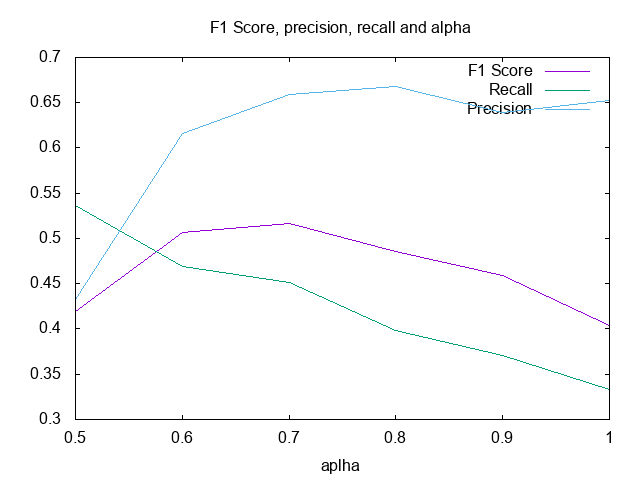
\includegraphics[width=0.6\textwidth]{40.png}
\caption{\label{fig:F1 Score, precision, recall and $\alpha$}F1 Score, precision, recall and $\alpha$}
\end{figure}


\item 
The graph below represents how F1 score varies with $\alpha$ and number of samples taken from Bloom Filter (with number of samples: 40, number of nodes: 100K and size of bloom filter: 200K).

\begin{figure}[H] 
\centering
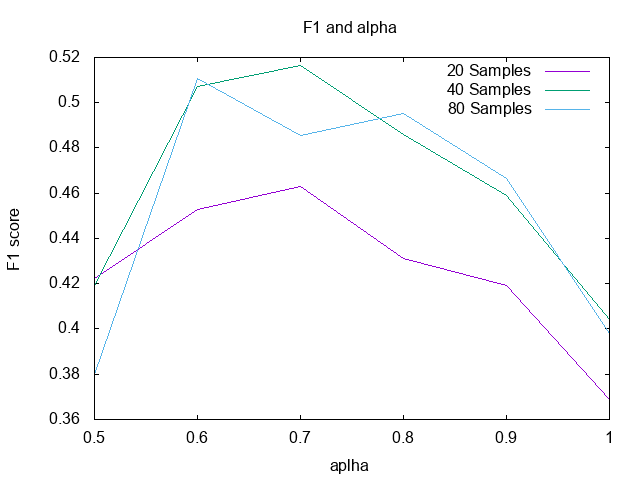
\includegraphics[width=0.6\textwidth]{F1.png}
\caption{\label{fig:F1 Score and $\alpha$}}
\end{figure}



\end{enumerate}

\clearpage
\bibliographystyle{alpha}
\bibliography{sample}
\end{document}